\documentclass{udpreport}
\title{Creación de paquetes utilizando Scapy y validación con Wireshark}
\author{Integrantes: Thomas Muñoz, Ignacio Yanjari, Dagoberto Navarrete, Ignacio López.}
\date{14 de Abril de 2016}
\usepackage{graphicx}
\usepackage{float}
\graphicspath{ {img/} }
\udpschool{Escuela de Informática y Telecomunicaciones}

\begin{document}
\maketitle
\tableofcontents
\chapter{Introducción}
	En este laboratorio buscamos aprender cómo se crean los paquetes con Scapy y como se organizan estos, además de entender la
	diferencia entre enviar un paquete a un equipo específico o a todos los pertenecientes a la red, a su vez entendimos la
	utilidad de Wireshark al tener que filtrar y capturar los paquetes que enviábamos entre nuestros equipos para verificar que se
	hayan recibido correctamente y estos no tuvieran algún tipo de problema.
\chapter{Actividades}
	\section{Instalacion de software}

	\section{Creacion de Paquetes}
		Para la creación de paquetes fue necesario aplicar nuestros conocimientos sobre la composición de un frame.
		Los frames cuentan con un Preámbulo el cual lleva una secuencia específica de bits para que el receptor note si el
		frame llega en buen estado o no, cuenta con un Delimitador de inicio el cual avisa al receptor que luego de una
		secuencia definida de unos y ceros se dará inicio a la información del frame, también cuenta con la dirección de
		destino y origen (MAC e IP), más adelante vienen unos bits donde se le da a conocer al receptor el largo de los datos
		del frame, para luego continuar con el Encabezado y datos reales del frame (mensaje) y para finalizar la trama hay una
		Secuencia de verificación donde se vuelve a evaluar que esta esté sin errores.\\
		\begin{figure}[H]
		    \centering
		    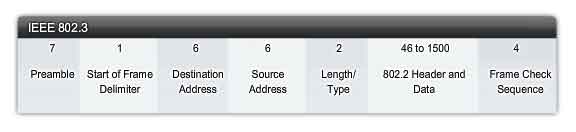
\includegraphics[width=\textwidth]{frame.jpg}
		    \caption{Frame según el estandar IEEE 802.3}
		    %\label{fig:my_label}
		\end{figure}
\chapter{Switch VS Hub}
	\section{Switch}
		Exite una gran diferencia entre enviar paquetes en equipos conectados a un switch, y en equipos conectados a un hub. a
		continuación se describirán los pasos llevados a cabo para enviar paquetes entre equipos conectados a un switch\\
		{\bf \large Envío Broadcast}\\
		Lo primero que hacemos es verificar la Mac y la IP de los equipos que vamos a utilizar, esto se hace a través del
		comando “ifconfig”. Ya una vez conocida la IP y la Mac de los equipos se procede a la creación de los paquetes, lo
		primero que debemos hacer es crear una variable y asignarle el comando “Ether()”, el cual trabaja en la segunda capa
		del modelo OSI (capa de enlace), después se la asigna un valor a la componente “dst” y “src”, estos valores son la Mac
		de destino
		y la de origen respectivamente, para la de destino se usó “ff:ff:ff:ff:ff:ff” ya que era una transmisión de tipo
		Broadcast. Después se crea otra variable a la cual se le asignará el comando “IP()”, el cual trabaja en la tercera
		capa del modelo OSI (capa de red), para esta variable se modificarán nuevamente las componentes “dst” y “src”, estas
		componentes corresponden a la IP de destino y a la de origen respectivamente, a “dst” se le asignara “255.255.255.255"
		, se le asigna este valor ya que se quiere hacer una transmisión de tipo Broadcast, mientras que al componente “src”
		se le asigna la IP del equipo que envia el paquete. Posteriormente se crea una nueva variable y a esta se le asigna el
		comando “ICMP()” el cual trabaja en la cuarta capa del modelo OSI (capa de transporte). Continuando se crea otra
		variable y a esta se le asigna el comando “Raw()”, una vez hecho todo lo anterior se crea una nueva variable (nuestro
		paquete)  y se le asignan las variables anteriores separadas de un “/” en el mismo orden que fueron nombradas.
		Finalmente se procede a enviar el paquete usando el comando “sendp“, ya que este comando sirve para enviar paquetes
		que van desde la segunda capa, una vez enviado el paquete se verifica que se recibido en todos los equipos que
		estábamos utilizando. Después creamos otro paquete pero este no incluía la variable asociada al comando “Ether()”,
		este paquete lo enviamos con el comando “send” ya que este trabaja con paquetes desde la tercera capa en adelante, una
		vez realizado lo anterior se comprueba que el paquete sea recibido en todos los equipos que estábamos utilizando.
		Todas las comprobaciones que se realizaban se hacían gracias al programa “wireshark” el cual nos permitía observar los
		paquetes que entraban y salían del ordenador.\\
		{\bf \large Envío a otro equipo}\\
		Para la creación de un paquete enviado a una dirección Mac específica y una IP correspondiente a la de un equipo de la
		red, se vuelven a crear nuevas variables y se le asignarán los comandos: “Ether()”, “IP()”, “ICMP()” y “Raw()”, pero
		esta vez cambiaremos la componente “dst” de “Ether()” por la dirección Mac del equipo que deseamos enviar los paquetes
		y la componente “dst” asociada al comando “IP()”, a esta se le asignara la dirección IP del equipo al que deseamos
		enviar el paquete. Ahora continuaremos con la creación de los paquetes, si deseamos enviar el paquete con el comando
		“send” solo será necesario apilar todas las variables con sus comandos asociados, excepto la variable asociada al
		comando “Ether()” puesto que esta no es necesaria con este comando debido a que este trabaja a partir de la tercera
		capa del modelo OSI, luego se procede a enviar el paquete y  después al revisar con wireshark se observa que
		efectivamente llega el paquete al equipo de destino. Mientras que si deseamos enviar el paquete con el comando “sendp”
		apilaremos todas las variables con sus respectivos comandos asociados,  pero esta vez se deberá enviar 2 veces el
		paquete, ya que la primera vez hará una transmisión tipo Broadcast para encontrar la IP del equipo de destino, y el
		segundo envio solo llegará al equipo de destino, esto se observa en la captura de paquetes que hizo wireshark en el
		equipo destinatario.\\
		{\bf \large Envío Mac inexistente}\\
		A continuación para enviar un paquete con la Mac errónea, se procede hacer los mismos procesos anteriormente
		mencionados, se vuelven a crear variables y se le asocia a cada una los comandos mencionados los en párrafos
		anteriores. Esta vez se modificara la Mac de destino (“dst”)  por una Mac de un equipo que no esté conectado a la red
		del laboratorio. Después se volverá a apilar todas las variables en el paquete que deseamos enviar, luego el paquete
		será enviado con el comando “sendp” ya que este trabaja con la segunda capa del modelo OSI, por lo que se verá
		obligado a trabajar con nuestra Mac errónea. Una vez enviado el paquete se procede a verificar en Wireshark, al
		observarlo nos damos cuenta de que el paquete enviado, al no encontrar la Mac de destino procede a hacer una
		transmisión de tipo Broadcast y envía el paquete a todos los equipos conectados a la red.\\
	\section{Hub}\\
	 	Al mandar paquetes en la red por medio de un HUB estos paquetes siempre 
 		le llegaran a todos los dispositivos conectados a la red.Mientras que si
 		se mandaran paquetes como por intermedio de un switch estos dependerian de 
 		las direcciones de destino  y sus comandos caracteristicos.\\
 		{\bf \large Envio Broadcast}\\
 		*Al momento de querer generar un broadcast en un HUB simplemente es tan facil como mandar
		paquete con direccion src y ip src desde el pc que uno este ocupando y este llegara a cada
 		dispositivo de nuestra red.\\
 		{\bf \large Envio  otro equipo}\\
 		{\bf \large Envio Mac inexistente}\\


	\section{Cuestionario}
	
	  1.-¿Qué pasa cuando envío un paquete a la dirección FF:FF:FF:FF:FF:FF? ¿Quienes
	     lo reciben? ¿Por qué?\\
    	 	\begin{figure}[H]
	        	\centering
	        	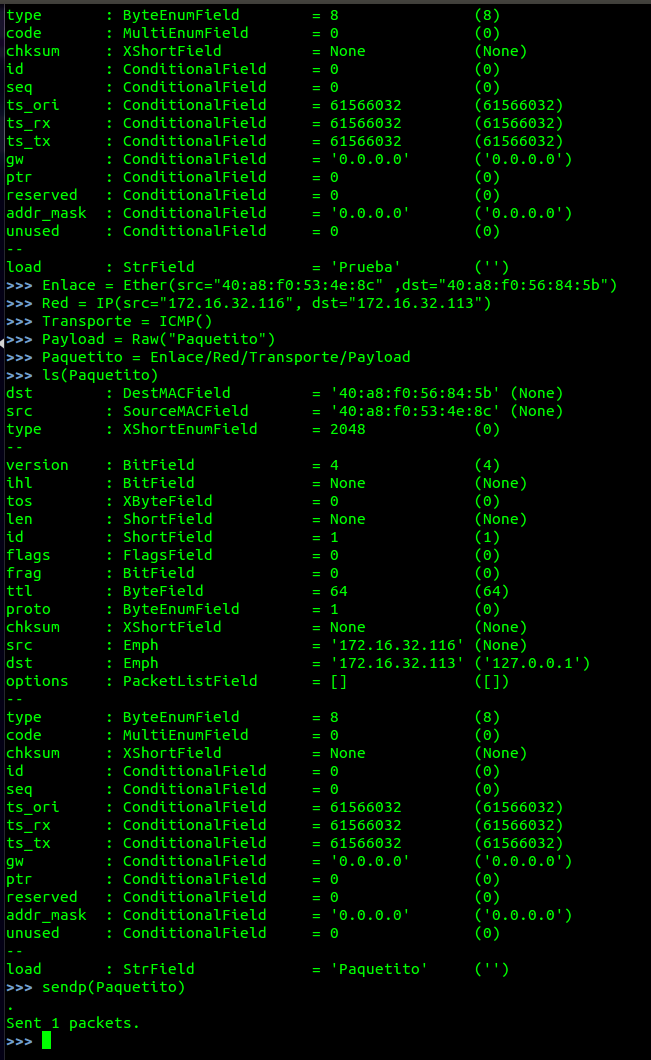
\includegraphics[width=10cm, height=11cm]{EnvioPaquetito.png}
			\caption{Envío en Broadcast}
	        	% \label{fig:my_label} %aun no se para que se usa pero se ve util
	 	\end{figure}
	     Cuando enviamos un paquete a la dirección FF:FF:FF:FF:FF:FF, este fue enviado a todos los equipos dentro de la red
	     Ethernet. Esto es debido a que la dirección antes mencionada esta designada para que la difusión de nuestro paquete sea
 	     enviado a cada dispositivo conectado a nuestra red LAN, a este tipo de difusión se le conoce como “Broadcast”.\\
 
  	  2.-¿Qué pasa cuando envío un paquete a una MAC de otro equipo? ¿Quienes lo
  	      pueden recibir? ¿Por qué?\\
    		\begin{figure}[H]
  	        	\centering
  	          	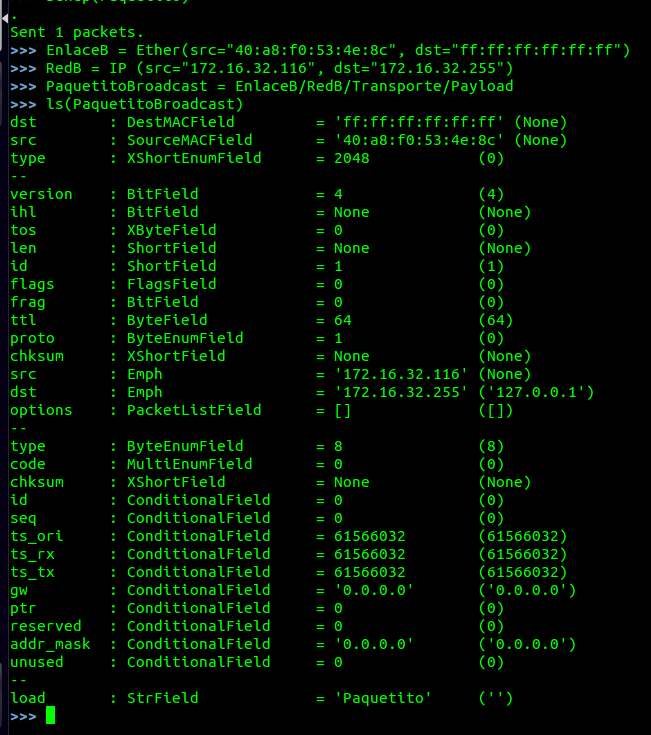
\includegraphics[width=10cm, height=11cm]{EnvioPaquetitoMalo2.png}
  	          	\caption{Envío a una MAC}
  	          	%\label{fig:my_label}
  		\end{figure}
 	      
 	      Cuando enviamos un paquete a la dirección MAC de otro equipo dentro de la red Ethernet, solamente el equipo que poseía
 	      esa dirección fue capaz de recibirlo. Esto ocurre puesto a que, como indicamos anteriormente, al paquete le dimos una
 	      MAC de destino fija, entonces el paquete se encargó de viajar solamente al equipo que poseía esa dirección\\
 
  	  3.-¿Qué sucede si envía un paquete a una MAC que no corresponda a ningún equipo
  	      de la red? ¿Quienes lo pueden recepcionar? ¿Por qué?\\
    		\begin{figure}[H]
  	        	\centering
  	          	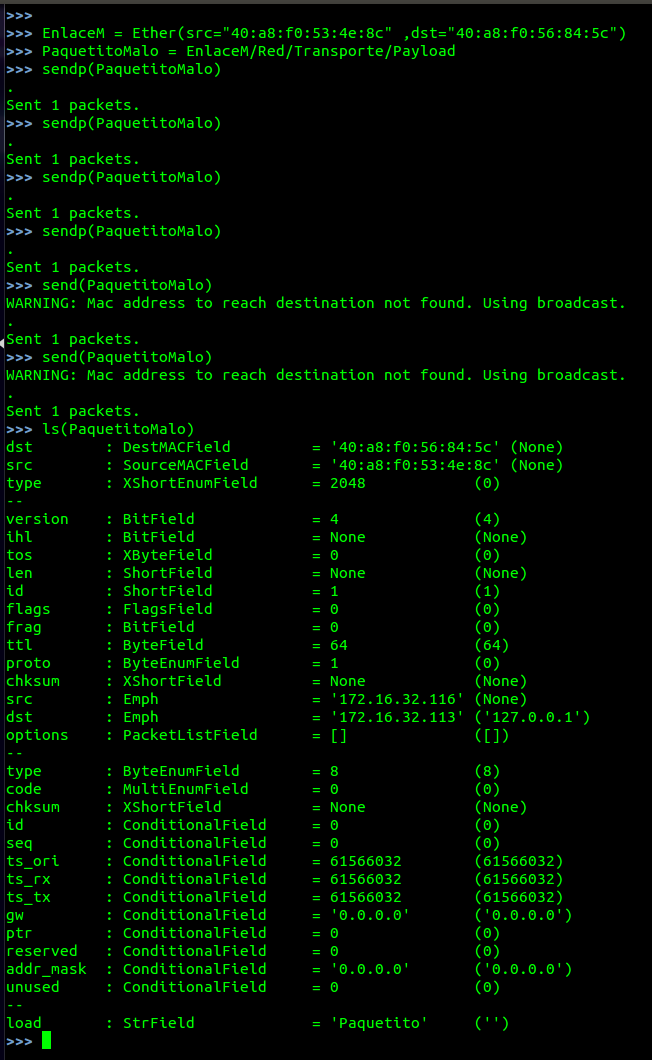
\includegraphics[width=10cm,height=11cm]{EnvioPaquetitoMalo.png}
  	        	\caption{Envío a una MAC fuera de la red}
  	            	%\label{fig:my_label}
  	        \end{figure}
 	      Cuando enviamos 
 	      Cuando enviamos un paquete a una dirección MAC que no correspondía a ningún equipo de la red, al enviarlo nos apareció
 	      el mensaje: “WARNING: Mac address to reach destination not found. Using Broadcast.” Y posteriormente el paquete fue
 	      enviado a todos los equipos pertenecientes a la red Ethernet. Se usa el Broadcast para así poder obtener todas las
 	      direcciónes MAC mediante su IP, registrarlas en la lista arp y encontrar la que se dio como destinataria, pero como esta
 	      no se encuentra en la red sigue mandando el paquete a todos los equipos que si están en la red para seguir buscando la
 	      MAC solicitada.\\

 	     
	      

\chapter{Conclusión}
  	      En esta experiencia de laboratorio se logra comprender cómo crear correctamente un paquete con Scapy,
  	      entendiendo todos sus componentes y cómo se puede enviar al o a los destinatarios que nosotros deseemos, también
  	      logra dejar clara la diferencia entre los comandos “send()” y “sendp()”, la capa en la que trabajan y cuando usar cada
  	      uno,se capta la forma en como funciona un Switch y un Hub con respecto al envío de paquetes y se aprendió trabajar con
  	      Wireshark para encontrar los paquetes del tipo que queramos o provenientes de la IP que cada uno  escoja.
\begin{thebibliography}{x}

\end{thebibliography}
\end{document}
